\renewcommand{\theequation}{\theenumi}
\begin{enumerate}[label=\arabic*.,ref=\thesubsection.\theenumi]
\numberwithin{equation}{enumi}
\item given that $\to$
\\
No of cases = 1000
\\
No of cases when the tyre lasts more than 9000 Km = $325 +445$ = 770
\\
probability of a tyre lasts more than 9000  Km = $P(X>9K)$
\begin{align}
P\left(X>9K\right) &= \frac{770}{1000}
\\
&=0.77
\end{align}
\item No of cases when the tyre lasts betwwen  4000 to 14000 Km = 20+210+325=555
\\
probability of a tyre lasts between 4000 to 14000 Km = $P(4K<X<14K)$
\begin{align}
P\left(4K<X<14K\right) &= \frac{555}{1000}
\\
&=0.0.555
\end{align}
\item No of cases when the tyre lasts less than 4000 Km = 20
\\
probability of a tyre lasts less than 4000 Km = $P(X<4K)$
\begin{align}
P\left(X<4K\right) &= \frac{20}{1000}
\\
&=0.02
\end{align}
codes for the above equation can be get from here
\begin{lstlisting}
codes/probexm/probexm6.py
\end{lstlisting}
\begin{figure}[!ht]
	\centering
	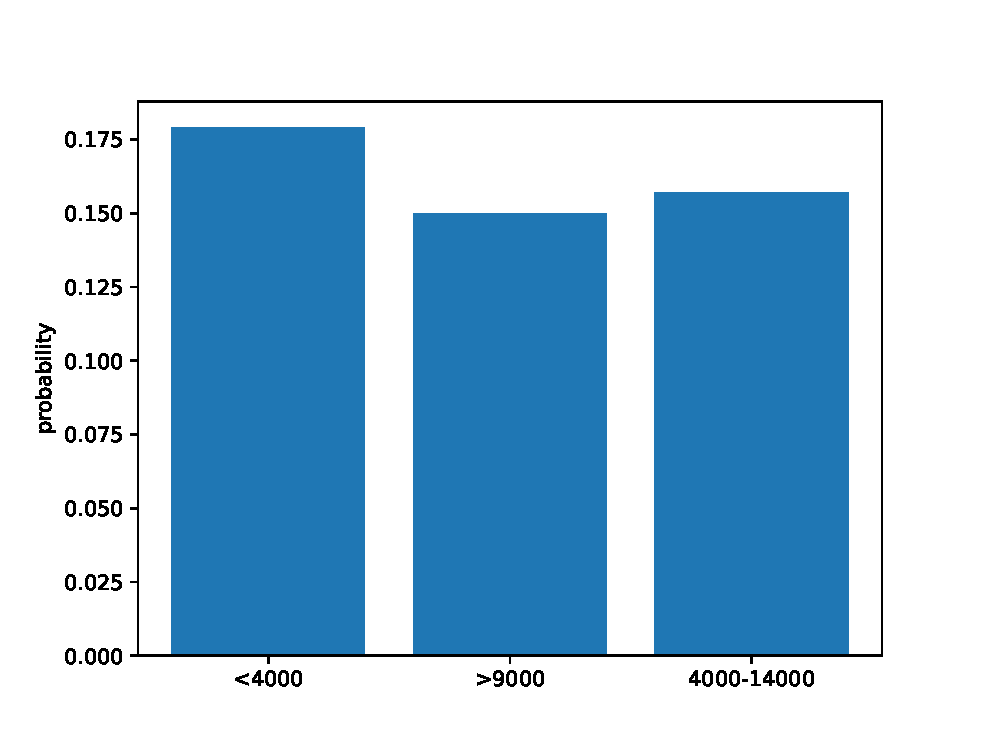
\includegraphics[width=\columnwidth]{./figures/probexm/probexm6.eps}
	\caption{probability of distance covered by tyre }
	\label{fig:bt6}
	\begin{lstlisting}
	figs/probexm/probexm6.eps
	\end{lstlisting}
\end{figure}
\end{enumerate}